\chapter{Resultados}
\label{cap:resultados}

\section{Caracterización de la cohorte}

La cohorte de análisis comprende $n=\cohorteN$ casos COVID confirmados del año
2021 --de \nBaseCompleta{} registros de notificación en el corte anual-- con una
mortalidad observada de \cohorteTasaDef\,\% y una tasa de hospitalización de
\tasaHospCohorte\,\%. A modo de contraste, la mortalidad sobre la base completa,
que incluye casos negativos y sospechosos, es de \tasaDefBase\,\%: la restricción
a casos confirmados no es un detalle de filtrado, sino la diferencia entre dos
poblaciones con riesgo basal muy distinto.

La calidad del dato es alta en las variables clave: la edad tiene
\faltEdad\,\% de valores faltantes y el sexo y la entidad de residencia están
completos. En las comorbilidades, la proporción de códigos de ausencia (97--99)
oscila entre \naComorbMin\,\% y \naComorbMax\,\%, con el máximo en
\texttt{\naComorbMaxVar}.

Esa ausencia no es ruido aleatorio, lo que justifica conservarla en lugar de
imputarla. En nueve de las once comorbilidades, los registros con código de
ausencia tienen una mortalidad hasta \naRazonMax{} veces mayor que los que sí
están codificados: en \texttt{\naVarMax}, \naMortConNa\,\% frente a
\naMortSinNa\,\%. En \texttt{\naVarMin} la relación se invierte por completo
(razón \naRazonMin), lo que es coherente con que sea el predictor dominante: no
registrar neumonía acompaña a los casos leves. Además su frecuencia difiere enormemente entre
estados: la máxima proporción de faltantes por entidad va de \naEntMin\,\% en
\naEntMinEnt{} a \naEntMax\,\% en \naEntMaxEnt. Es, por tanto, un mecanismo
plausible de inequidad geográfica que este trabajo documenta pero no explota: los
indicadores de ausencia no se usan como predictores (apéndice~\ref{ap:variables}).

La figura~\ref{fig:eda} muestra la heterogeneidad que motiva la tesis. El tamaño
de muestra por entidad varía por un factor de \entFactorN{} --de \entNmin{} a
\entNmax{} registros-- y las tasas de defunción difieren por un factor de
\entFactorTasa{} entre los extremos. Esa doble heterogeneidad --de volumen y de
riesgo basal-- es la condición de la que cabe esperar desempeño desigual.

\begin{figure}[htbp]
\centering
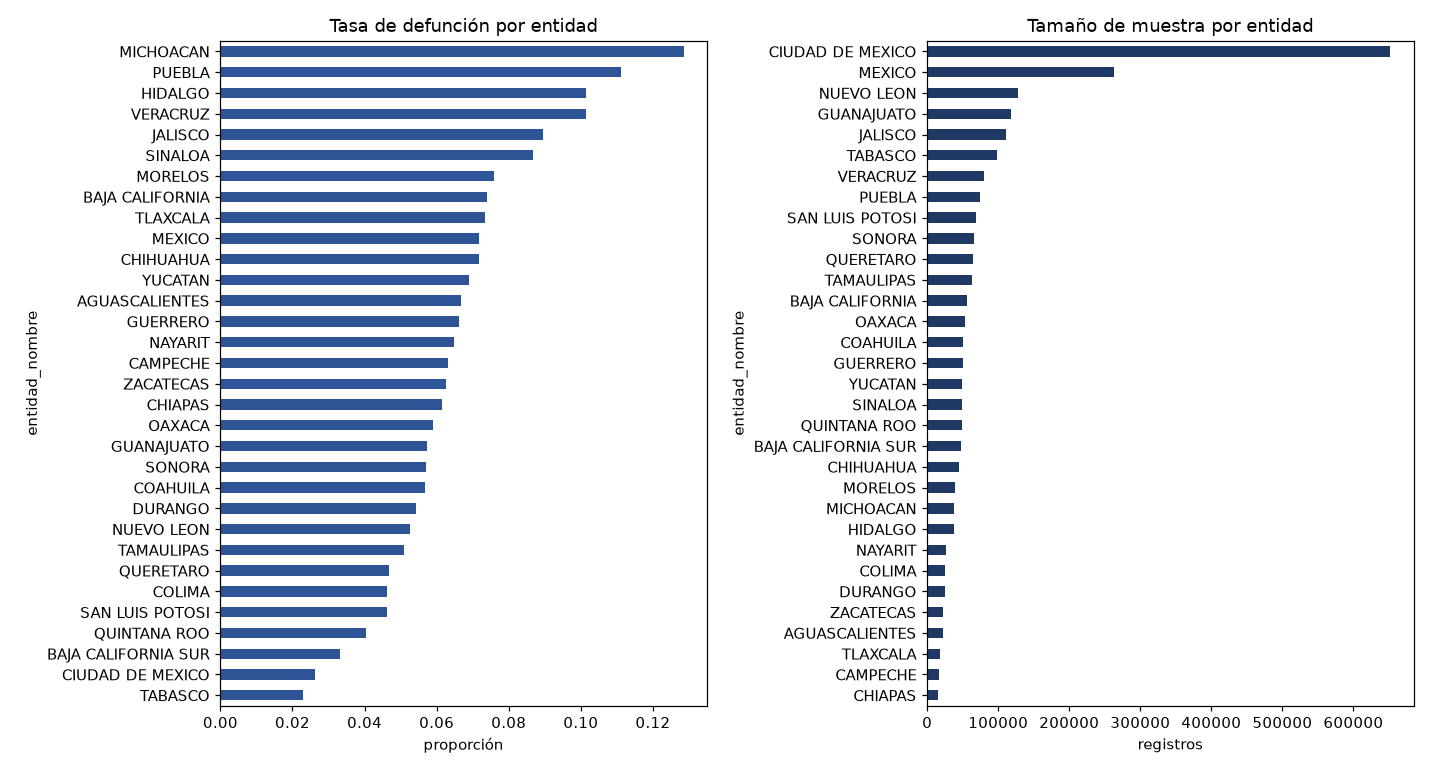
\includegraphics[width=\linewidth]{eda_por_entidad.png}
\caption{Heterogeneidad entre entidades federativas en la cohorte: tasa de
defunción (izquierda) y tamaño de muestra (derecha).}
\label{fig:eda}
\end{figure}

\section{Desempeño del modelo de referencia}

El modelo principal alcanza un \textbf{AUROC de \aurocGlobal} y un AUPRC de
\auprcGlobal{} sobre el conjunto de prueba ($n=\testN$), entrenado sobre
\nTrain{} registros y calibrado sobre \nCalib. La regresión logística
obtiene un AUROC de \logitAUROC, apenas por debajo, lo que indica que la señal
disponible en edad, sexo y comorbilidades es en buena medida lineal y que el
impulso del gradiente aporta poco en discriminación.

La comparación con la literatura sobre esta misma base debe hacerse con cautela,
porque los trabajos de referencia reportan exactitud y $F_1$ y no
AUROC~\parencite{becerra2022,mendez2024}, de modo que las cifras no son
directamente homologables. Lo que sí puede afirmarse es que el modelo no está
deliberadamente debilitado: usa los predictores habituales de esa literatura, un
algoritmo del mismo tipo y una cohorte de la misma fuente, y coincide con ella en
qué variables resultan más informativas (sección~\ref{sec:importancia}). Eso basta
para el propósito de la línea de base, que es que el sujeto de la auditoría sea un
modelo razonable y no un espantapájaros.

\subsection{Efecto de la calibración}

El modelo sin calibrar discrimina bien pero está severamente descalibrado: emite
un riesgo medio de \crudoRiesgo{} frente a una mortalidad observada de
\mortObsTest, es decir una sobreestimación por un factor de
\factorSobreestimacion, consecuencia directa de la reponderación por clase. La regresión isotónica ajustada sobre el
bloque de calibración reduce el puntaje de Brier de \brierCrudo{} a
\brierCalibrado{} y alinea el riesgo medio predicho (\calibRiesgo) con el
observado, dejando el AUROC esencialmente intacto --\aurocGlobal{} frente a
\crudoAUROC-- como corresponde a una transformación monótona.

\nota{Este resultado tiene una consecuencia que va más allá del ajuste. Una
auditoría de calibración por grupo realizada sobre el puntaje sin calibrar habría
reportado un error máximo de calibración por entidad de \errCalCrudo, cifra que
corresponde casi enteramente al sesgo global de entrenamiento y no a la inequidad
geográfica. Medida sobre el riesgo calibrado, la misma métrica es \errCalEntidad.
La conclusión sustantiva se invierte: la calibración por entidad, una vez
corregido el nivel global, es \emph{buena}.}

\subsection{Importancia de variables}
\label{sec:importancia}

La importancia por permutación sobre el AUROC (tabla~\ref{tab:importancia})
concentra la señal en dos variables: \texttt{\impPrimeraVar} (\impPrimera) y la
edad (\impSegunda). El resto de los predictores aporta \impTercera{} o menos cada
uno. La concentración es coherente con la literatura sobre esta
base~\parencite{becerra2022}, y refuerza la advertencia de la
sección~\ref{sec:fuga}: la validez del modelo depende de que la neumonía esté
efectivamente registrada al primer contacto.

% Generado por generar_tablas.py -- NO editar a mano.

\begin{table}[htbp]
\centering
\small
\caption{Importancia por permutación sobre el AUROC en el conjunto de prueba
(3 repeticiones, submuestra de \numprint{50000} observaciones).}
\label{tab:importancia}
\begin{tabular}{l r}
\toprule
Variable & Caída de AUROC \\
\midrule
NEUMONIA & 0.1057 \\
EDAD & 0.0789 \\
sexo\_mujer & 0.0029 \\
DIABETES & 0.0028 \\
RENAL\_CRONICA & 0.0016 \\
OBESIDAD & 0.0011 \\
OTRA\_COM & 0.0010 \\
HIPERTENSION & 0.0009 \\
INMUSUPR & 0.0002 \\
TABAQUISMO & 0.0001 \\
CARDIOVASCULAR & 0.0001 \\
EPOC & 0.0000 \\
ASMA & 0.0000 \\
\bottomrule
\end{tabular}
\end{table}


\section{Auditoría de equidad}

Todas las métricas dependientes de umbral se evalúan en el punto de operación
común $\tau=\umbralOperacion$, que alcanza una sensibilidad global de
\tprObjetivo{} con una tasa de falsos positivos de \fprObjetivo.

\subsection{Entidad federativa}

La tabla~\ref{tab:entidad} presenta el desempeño por entidad, la
tabla~\ref{tab:disparidad} resume las brechas por eje de auditoría y la
figura~\ref{fig:equidad} las visualiza. El hallazgo
central es una \textbf{disparidad geográfica sustantiva}: la sensibilidad varía
\gapTPRentidad{} entre entidades y el AUROC \gapAUROCentidad. El peor desempeño
corresponde a \entPeor{} (AUROC \entPeorAUROC, sensibilidad \entPeorTPR) y el
mejor a \entMejor{} (AUROC \entMejorAUROC, sensibilidad \entMejorTPR).

La magnitud merece leerse en términos clínicos y no estadísticos. Con un umbral
único calibrado para detectar al \sensObjetivo\,\% de las defunciones a nivel
nacional, el modelo detecta cerca de \entPeorPct{} de cada 100 en la entidad peor
servida y \entMejorPct{} de cada 100 en la mejor servida. La diferencia --unas
\entDifPct{} defunciones no priorizadas por cada 100-- recae sobre la población de un estado concreto por el solo hecho de residir
en él.

% Generado por generar_tablas.py -- NO editar a mano.

\begin{table}[htbp]
\centering
\caption{Brechas máximas entre grupos por eje de auditoría, al umbral
$\tau=0.1562$. La brecha de TPR corresponde a la violación de
\emph{equalized odds}; el error de calibración se mide sobre el riesgo calibrado.}
\label{tab:disparidad}
\small\setlength{\tabcolsep}{5pt}
\begin{tabular}{l r r r r r}
\toprule
Eje & $\Delta$TPR & $\Delta$FPR & $\Delta$AUROC & $\Delta$Selec. & Err.\ calib. \\
\midrule
Entidad federativa & 0.2935 & 0.0867 & 0.0563 & 0.1556 & 0.0231 \\
Sexo & 0.0393 & 0.0268 & 0.0082 & 0.0448 & 0.0005 \\
Grupo etario & 0.5824 & 0.3026 & 0.0903 & 0.4408 & 0.0008 \\
\bottomrule
\end{tabular}
\end{table}

% Generado por generar_tablas.py -- NO editar a mano.

\begingroup
\small\setlength{\tabcolsep}{4pt}
\begin{longtable}{l r r r r r r}
\caption{Desempeño y equidad por entidad federativa en el conjunto de prueba
($n=631\,663$), al umbral de sensibilidad objetivo
$\tau=0.1562$. Ordenadas por AUROC ascendente.}
\label{tab:entidad}\\
\toprule
Entidad & $n$ & Mort. & AUROC & TPR & FPR & Riesgo \\
\midrule
\endfirsthead
\toprule
Entidad & $n$ & Mort. & AUROC & TPR & FPR & Riesgo \\
\midrule
\endhead
\midrule
\multicolumn{7}{r}{\footnotesize Continúa en la página siguiente} \\
\endfoot
\bottomrule
\endlastfoot
Chihuahua & 11\,072 & 0.0713 & 0.9207 & 0.688 & 0.081 & 0.0659 \\
Chiapas & 3\,831 & 0.0611 & 0.9265 & 0.662 & 0.065 & 0.0567 \\
Baja California Sur & 11\,712 & 0.0307 & 0.9272 & 0.683 & 0.040 & 0.0347 \\
Aguascalientes & 5\,498 & 0.0615 & 0.9304 & 0.657 & 0.060 & 0.0532 \\
Durango & 6\,297 & 0.0569 & 0.9310 & 0.631 & 0.052 & 0.0465 \\
Veracruz & 20\,275 & 0.1012 & 0.9340 & 0.766 & 0.086 & 0.0826 \\
Nuevo León & 32\,110 & 0.0528 & 0.9341 & 0.686 & 0.046 & 0.0449 \\
Coahuila & 12\,615 & 0.0576 & 0.9342 & 0.686 & 0.054 & 0.0502 \\
Jalisco & 27\,918 & 0.0887 & 0.9348 & 0.703 & 0.067 & 0.0656 \\
Michoacán & 9\,484 & 0.1281 & 0.9359 & 0.853 & 0.116 & 0.1114 \\
México & 65\,705 & 0.0720 & 0.9387 & 0.760 & 0.070 & 0.0634 \\
Tlaxcala & 4\,288 & 0.0702 & 0.9391 & 0.841 & 0.100 & 0.0780 \\
Sinaloa & 12\,274 & 0.0849 & 0.9394 & 0.799 & 0.076 & 0.0735 \\
Nayarit & 6\,700 & 0.0710 & 0.9402 & 0.700 & 0.049 & 0.0537 \\
Hidalgo & 9\,345 & 0.1022 & 0.9410 & 0.881 & 0.123 & 0.1011 \\
Zacatecas & 5\,534 & 0.0614 & 0.9431 & 0.773 & 0.067 & 0.0591 \\
Yucatán & 12\,490 & 0.0705 & 0.9440 & 0.726 & 0.048 & 0.0515 \\
Puebla & 18\,800 & 0.1130 & 0.9480 & 0.920 & 0.118 & 0.1083 \\
Oaxaca & 13\,461 & 0.0558 & 0.9512 & 0.792 & 0.060 & 0.0560 \\
Querétaro & 16\,305 & 0.0449 & 0.9530 & 0.816 & 0.055 & 0.0497 \\
Tamaulipas & 15\,876 & 0.0544 & 0.9539 & 0.809 & 0.048 & 0.0509 \\
Campeche & 4\,191 & 0.0625 & 0.9544 & 0.920 & 0.111 & 0.0837 \\
Guanajuato & 29\,653 & 0.0575 & 0.9579 & 0.833 & 0.061 & 0.0586 \\
Baja California & 13\,953 & 0.0754 & 0.9584 & 0.887 & 0.080 & 0.0782 \\
Colima & 6\,390 & 0.0444 & 0.9598 & 0.824 & 0.052 & 0.0496 \\
Morelos & 9\,756 & 0.0763 & 0.9600 & 0.914 & 0.095 & 0.0875 \\
Ciudad de México & 162\,746 & 0.0262 & 0.9607 & 0.808 & 0.040 & 0.0367 \\
Quintana Roo & 12\,151 & 0.0414 & 0.9623 & 0.813 & 0.041 & 0.0393 \\
Sonora & 16\,698 & 0.0562 & 0.9628 & 0.868 & 0.064 & 0.0621 \\
San Luis Potosí & 17\,326 & 0.0459 & 0.9647 & 0.868 & 0.057 & 0.0528 \\
Guerrero & 12\,589 & 0.0666 & 0.9679 & 0.925 & 0.080 & 0.0751 \\
Tabasco & 24\,620 & 0.0222 & 0.9770 & 0.879 & 0.036 & 0.0348 \\
\end{longtable}
\endgroup


\begin{figure}[htbp]
\centering
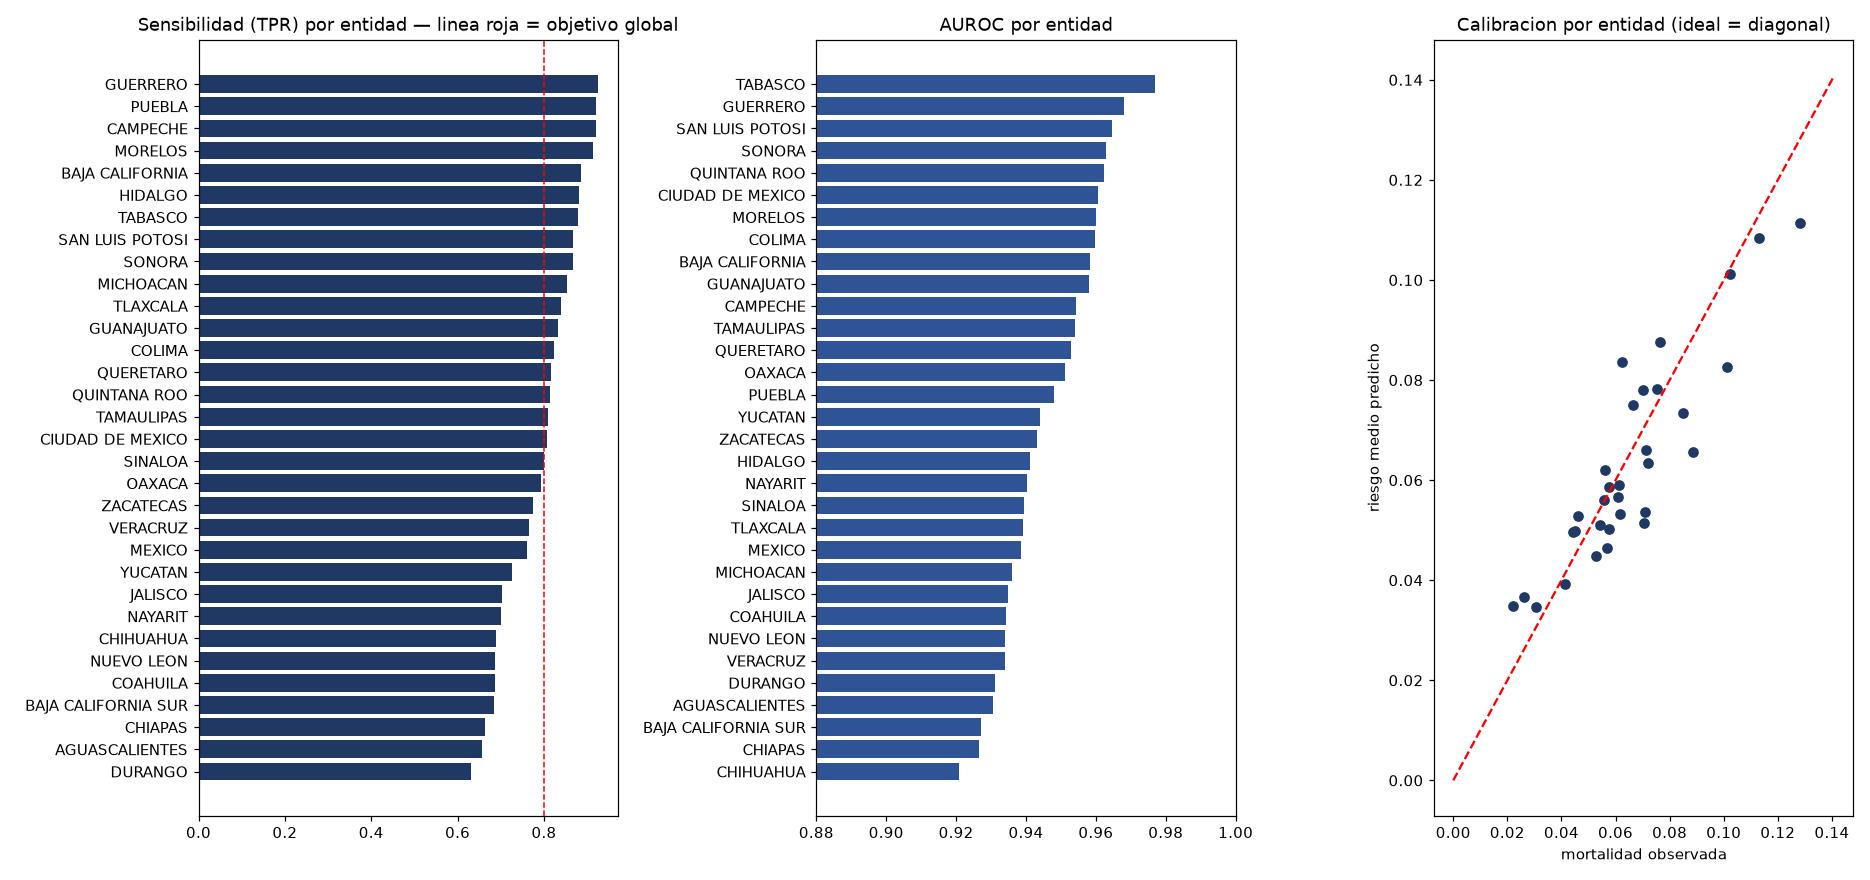
\includegraphics[width=\linewidth]{equidad_por_entidad.png}
\caption{Auditoría por entidad federativa: sensibilidad frente al objetivo global
(izquierda), AUROC (centro) y calibración, riesgo medio predicho frente a
mortalidad observada (derecha).}
\label{fig:equidad}
\end{figure}

Conviene notar la disociación entre criterios de equidad. El error máximo de
calibración por entidad es \errCalEntidad, es decir, la probabilidad emitida
significa aproximadamente lo mismo en cada estado; sin embargo la brecha de
sensibilidad es \gapTPRentidad. Un modelo puede estar bien calibrado en todos los
grupos y repartir la sensibilidad de forma muy desigual: es exactamente el
comportamiento que anticipa el teorema de imposibilidad cuando las prevalencias
difieren entre grupos~\parencite{chouldechova2017,kleinberg2017}. Conviene
subrayar que la calibración es propiedad del puntaje y no de la regla de
decisión, de modo que el error de \errCalEntidad{} no se altera por ninguna
elección de umbral, incluida la mitigación de la
sección~\ref{sec:mitigacion_res}. El mecanismo es
directo: con un umbral fijo sobre un puntaje bien calibrado, la fracción de
positivos que quedan por encima del corte depende de la distribución de riesgo
dentro del grupo, y esa distribución es distinta en cada entidad.

\subsection{Incertidumbre de las brechas}
\label{sec:incertidumbre_res}

Las cifras anteriores son estimaciones puntuales sobre un único conjunto de
prueba. La tabla~\ref{tab:incertidumbre} añade intervalos de confianza al
95\,\% por remuestreo y la tabla~\ref{tab:permutacion} contrasta las brechas
contra su distribución bajo la hipótesis nula de que la entidad no influye
(sección~\ref{sec:incertidumbre}).

% Generado por generar_tablas.py -- NO editar a mano.

\begin{table}[htbp]
\centering
\small\setlength{\tabcolsep}{4pt}
\caption{Desempeño por entidad con intervalos de confianza al 95\,\% obtenidos
por remuestreo estratificado (1000 réplicas); cinco peores y cinco
mejores por AUROC.}
\label{tab:incertidumbre}
\begin{tabular}{l r r c r c}
\toprule
Entidad & $n$ & AUROC & IC 95\,\% & TPR & IC 95\,\% \\
\midrule
Chihuahua & 11\,072 & 0.9207 & [0.9125,\,0.9290] & 0.688 & [0.654,\,0.720] \\
Chiapas & 3\,831 & 0.9265 & [0.9116,\,0.9407] & 0.662 & [0.604,\,0.721] \\
Baja California Sur & 11\,712 & 0.9272 & [0.9135,\,0.9398] & 0.683 & [0.635,\,0.731] \\
Aguascalientes & 5\,498 & 0.9304 & [0.9182,\,0.9418] & 0.657 & [0.603,\,0.705] \\
Durango & 6\,297 & 0.9310 & [0.9190,\,0.9427] & 0.631 & [0.580,\,0.680] \\
\midrule
Quintana Roo & 12\,151 & 0.9623 & [0.9539,\,0.9699] & 0.813 & [0.777,\,0.845] \\
Sonora & 16\,698 & 0.9628 & [0.9582,\,0.9677] & 0.868 & [0.847,\,0.889] \\
San Luis Potosí & 17\,326 & 0.9647 & [0.9587,\,0.9701] & 0.868 & [0.844,\,0.891] \\
Guerrero & 12\,589 & 0.9679 & [0.9635,\,0.9720] & 0.925 & [0.907,\,0.943] \\
Tabasco & 24\,620 & 0.9770 & [0.9717,\,0.9820] & 0.879 & [0.851,\,0.907] \\
\bottomrule
\end{tabular}
\end{table}

% Generado por generar_tablas.py -- NO editar a mano.

\begin{table}[htbp]
\centering
\small
\caption{Prueba de permutación sobre las brechas entre entidades
(1000 permutaciones de las etiquetas de entidad, conservando
los tamaños de grupo). La brecha bajo la nula no es cero: con 32 grupos, máximo y
mínimo se separan por azar.}
\label{tab:permutacion}
\begin{tabular}{l r r r r}
\toprule
Brecha & Observada & IC 95\,\% & Nula (mediana) & $p$ \\
\midrule
AUROC & 0.0563 & [0.0496,\,0.0697] & 0.0175 & 0.001 \\
Sensibilidad & 0.2935 & [0.2671,\,0.3535] & 0.0737 & 0.001 \\
\bottomrule
\end{tabular}
\end{table}


\begin{figure}[htbp]
\centering
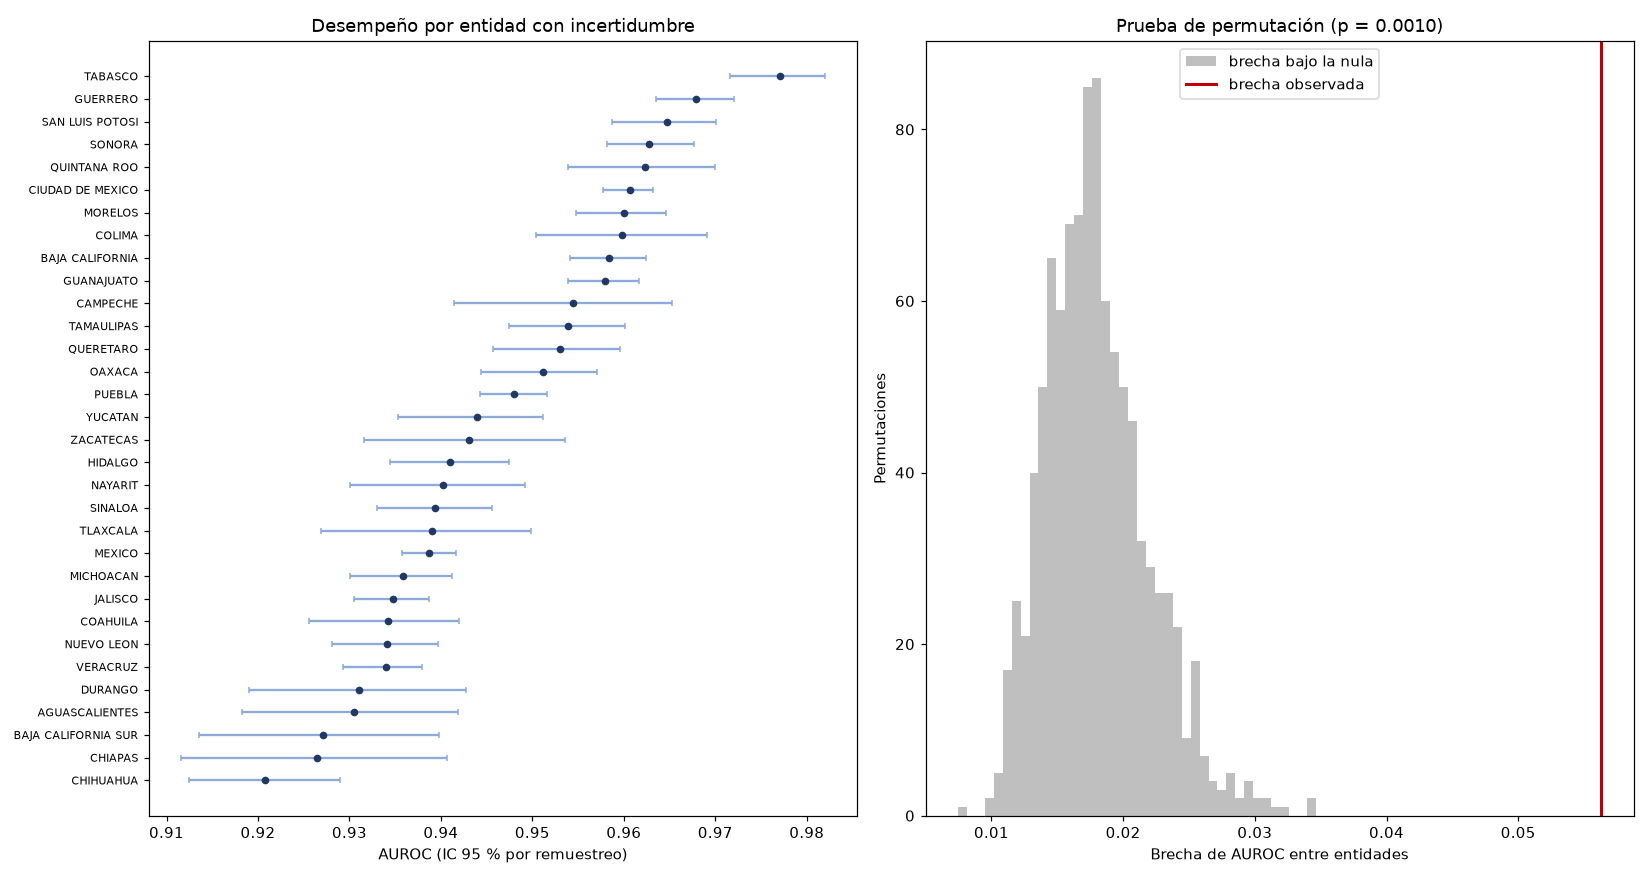
\includegraphics[width=\linewidth]{incertidumbre_brechas.png}
\caption{Izquierda: AUROC por entidad con intervalo de confianza al 95\,\%.
Derecha: distribución de la brecha de AUROC bajo la hipótesis nula de ausencia de
efecto de entidad, frente a la brecha observada.}
\label{fig:incertidumbre}
\end{figure}

El resultado más importante es que \textbf{las brechas bajo la nula no son cero}.
Permutando al azar las etiquetas de entidad, la brecha mediana de AUROC es
\nulaAuroc{} y la de sensibilidad \nulaTpr: con 32 grupos de tamaños desiguales,
el máximo y el mínimo se separan por azar sin que haya efecto alguno. Ese es el
punto de comparación correcto, y no el cero.

Contra esa referencia, las brechas observadas son claramente excesivas. La de
AUROC, \gapAUROCentidad{} (IC 95\,\%: \gapAurocICa--\gapAurocICb), supera el
percentil 95 de la nula (\nulaAurocPsup); la de sensibilidad, \gapTPRentidad{}
(IC 95\,\%: \gapTprICa--\gapTprICb), supera con holgura el suyo (\nulaTprPsup). En
ambos casos $p=\pAuroc$ y $p=\pTpr$ respectivamente, que es el mínimo alcanzable
con \boP{} permutaciones: ninguna reasignación al azar produjo una brecha tan
grande como la real.

Conviene traducir esto a la magnitud del efecto. De la brecha de sensibilidad
observada, alrededor de \nulaTpr{} es lo que el azar produce con esta estructura
de grupos; el exceso atribuible a la entidad es de aproximadamente \excesoTpr.
Sigue siendo grande, pero es la cifra honesta.

A nivel de entidad individual, \paresDisjuntos{} de los \paresTotal{} pares
posibles tienen intervalos de AUROC disjuntos (\paresPct\,\%), y los extremos
--\entPeor{} y \entMejor-- lo están. La precisión es razonable incluso en las
entidades pequeñas: el intervalo más ancho es el de \icAncho{} ($n=\icAnchoN$),
con una amplitud de \icAnchoAmp. El ordenamiento fino de la
tabla~\ref{tab:entidad} no debe leerse posición por posición, pero la separación
entre los extremos no es ruido.

\subsection{Sexo y grupo etario}

Las tablas~\ref{tab:sexo} y~\ref{tab:edad} presentan los otros dos ejes. El sesgo
por \textbf{sexo} es pequeño: la brecha de sensibilidad es \gapTPRsexo{} y la de
AUROC \gapAUROCsexo. El sesgo por \textbf{grupo etario} es el mayor de los tres
--brecha de sensibilidad \gapTPRedad{} y de AUROC \gapAUROCedad-- pero su
interpretación es distinta.

% Generado por generar_tablas.py -- NO editar a mano.

\begin{table}[htbp]
\centering
\small\setlength{\tabcolsep}{4pt}
\caption{Desempeño y equidad por sexo en el conjunto de prueba.}
\label{tab:sexo}
\begin{tabular}{l r r r r r r r}
\toprule
Sexo & $n$ & Mort. & AUROC & TPR & FPR & Selec. & Riesgo \\
\midrule
Hombre & 309\,437 & 0.0681 & 0.9456 & 0.811 & 0.073 & 0.123 & 0.0676 \\
Mujer & 322\,226 & 0.0444 & 0.9538 & 0.772 & 0.046 & 0.079 & 0.0444 \\
\bottomrule
\end{tabular}
\end{table}

% Generado por generar_tablas.py -- NO editar a mano.

\begin{table}[htbp]
\centering
\small\setlength{\tabcolsep}{4pt}
\caption{Desempeño y equidad por grupo etario en el conjunto de prueba.}
\label{tab:edad}
\begin{tabular}{l r r r r r r r}
\toprule
Grupo etario & $n$ & Mort. & AUROC & TPR & FPR & Selec. & Riesgo \\
\midrule
0-17 & 47\,676 & 0.0029 & 0.9347 & 0.266 & 0.003 & 0.004 & 0.0027 \\
18-39 & 303\,100 & 0.0089 & 0.9346 & 0.608 & 0.015 & 0.020 & 0.0089 \\
40-59 & 196\,593 & 0.0558 & 0.9039 & 0.743 & 0.062 & 0.100 & 0.0554 \\
60+ & 84\,285 & 0.2560 & 0.8444 & 0.849 & 0.306 & 0.445 & 0.2552 \\
\bottomrule
\end{tabular}
\end{table}


La brecha etaria es en buena medida mecánica y no debe leerse como inequidad en el
mismo sentido. La edad es el segundo predictor más informativo y las tasas base
difieren por dos órdenes de magnitud: \edadMenorTasa\,\% en menores de 18 años
frente a \edadMayorTasa\,\% en el grupo de 60 o más. Con un umbral único sobre un puntaje calibrado,
un grupo con riesgo basal muy bajo cae casi enteramente por debajo del corte, y su
sensibilidad se hunde por construcción: en 0--17 años es \edadMenorTPR{} con una
tasa de selección de \edadMenorSel\,\%. Igualar la sensibilidad entre grupos etarios exigiría
seleccionar una fracción mucho mayor de menores, con un valor predictivo positivo
muy bajo, algo difícil de justificar clínicamente. La disparidad geográfica no
admite esa explicación, porque las entidades no difieren en riesgo basal de forma
comparable ni la entidad es un predictor del modelo.

\subsection{Análisis interseccional}
\label{sec:interseccional}

Para descartar que la brecha geográfica sea un reflejo de la composición etaria de
cada estado, se repite la auditoría restringiendo la muestra a adultos de
\textbf{60 años o más} (tabla~\ref{tab:interseccional}). La disparidad no
desaparece: el AUROC varía de \sesentaPeorAUROC{} en \sesentaPeor{} a
\sesentaMejorAUROC{} en \sesentaMejor, un rango de \sesentaRango{} frente a
\gapAUROCentidad{} en la población completa.

% Generado por generar_tablas.py -- NO editar a mano.

\begin{table}[htbp]
\centering
\caption{Subgrupo interseccional: adultos de 60 años o más, por entidad
(cinco peores y cinco mejores de 32 evaluadas). El deterioro persiste
tras controlar por edad avanzada.}
\label{tab:interseccional}
\begin{tabular}{l r r r r}
\toprule
Entidad & $n$ & Mortalidad & AUROC & TPR \\
\midrule
Chiapas & 482 & 0.322 & 0.688 & 0.748 \\
Chihuahua & 1\,798 & 0.274 & 0.737 & 0.732 \\
Jalisco & 4\,212 & 0.382 & 0.758 & 0.771 \\
Aguascalientes & 730 & 0.311 & 0.763 & 0.771 \\
Veracruz & 3\,243 & 0.385 & 0.764 & 0.792 \\
\midrule
Campeche & 599 & 0.295 & 0.881 & 0.977 \\
San Luis Potosí & 2\,495 & 0.202 & 0.889 & 0.897 \\
Guerrero & 2\,046 & 0.277 & 0.889 & 0.951 \\
Ciudad de México & 20\,942 & 0.128 & 0.895 & 0.858 \\
Tabasco & 2\,801 & 0.117 & 0.942 & 0.930 \\
\bottomrule
\end{tabular}
\end{table}


Este es el resultado más consistente con la hipótesis~\ref{h1} en su formulación
fuerte: la inequidad geográfica es una propiedad del modelo y no un artefacto de
la estructura demográfica de las entidades.

Dos matices impiden sobreinterpretarlo. El primero es de precisión: los subgrupos
son pequeños --\sesentaPeor{} aporta apenas \sesentaPeorN{} observaciones-- de
modo que buena parte de la amplitud del rango es varianza de muestreo y no
inequidad estimada con fiabilidad. Los intervalos de confianza de la
sección~\ref{sec:incertidumbre_res} se calcularon sobre la población completa, no
dentro de este subgrupo, donde los tamaños son un orden de magnitud menores; para
él sigue sin haber una medida de precisión.

De hecho \sesentaPeor{} queda por debajo del criterio general de soporte, que se
relajó aquí a \interMinN{} observaciones (sección~\ref{sec:particion}). Aplicando
el criterio de \numprint{500} quedarían \interNestandar{} entidades, el peor
desempeño sería \interPeorEstandar{} con \interPeorEstandarAUROC{} y el rango
bajaría a \interRangoEstandar. La conclusión no depende de la elección: bajo
cualquiera de los dos criterios la dispersión dentro del subgrupo supera con
holgura la de la población completa (\gapAUROCentidad).

El segundo es que la ampliación del rango de AUROC dentro de los adultos mayores
matiza el diagnóstico de la sección~\ref{sec:mitigacion_res}. En la población
completa la disparidad reside claramente en el umbral y no en el ordenamiento;
dentro del subgrupo de 60 años o más, en cambio, la dispersión del AUROC es del
mismo orden que la de la sensibilidad, lo que sugiere que ahí también hay un
componente de ordenamiento. Si es así, una mitigación basada solo en umbrales
sería menos efectiva en ese subgrupo que en la población general. Comprobarlo
exige repetir la mitigación dentro del subgrupo, algo que este trabajo no hace.

Conviene además no leer el resultado en clave de marginación. El subgrupo con
peor discriminación (\sesentaPeor, grado «Muy alto») no es el de mayor mortalidad
--esa es \sesentaMasLetal, con \sesentaMasLetalTasa{} frente a
\sesentaPeorTasa-- y entre los cinco mejores figura Guerrero, la entidad con
mayor marginación del país. El patrón por grado de marginación se examina en la
sección~\ref{sec:correlatos} y no aparece.

\subsection{Correlatos de la inequidad geográfica}
\label{sec:correlatos}

Se examinó la asociación entre el desempeño por entidad y tres características
del grupo. Sobre las \nEntidades{} entidades:

\begin{itemize}[leftmargin=*]
  \item \textbf{Tamaño de muestra.} $r=\corrAurocNr$ ($p=\corrAurocNp$);
    Spearman $\rho=\corrAurocNrho$ ($p=\corrAurocNprho$). Asociación positiva
    débil y no significativa.
  \item \textbf{Tasa de mortalidad de la entidad.} $r=\corrAurocTasar$
    ($p=\corrAurocTasap$); $\rho=\corrAurocTasarho$ ($p=\corrAurocTasaprho$).
    Es la única asociación que alcanza significación convencional: el modelo
    discrimina peor en las entidades con mayor mortalidad observada.
  \item \textbf{Índice de marginación.} $r=\corrMargAurocr$
    ($p=\corrMargAurocp$); $\rho=\corrMargAurocrho$ ($p=\corrMargAurocprho$).
    Sin asociación detectable. Para la sensibilidad, $r=\corrMargTprr$
    ($p=\corrMargTprp$).
\end{itemize}

El índice de marginación procede del archivo por entidad de los \emph{Índices de
marginación 2020} de CONAPO, construidos sobre el Censo de Población y Vivienda
2020~\parencite{conapo2020}. Conviene precisar su escala, porque se presta a
confusión: la edición 2020 se calcula por Distancias Ponderadas al cuadrado y un
valor \emph{más alto} indica \emph{menor} marginación --Guerrero 10.99, grado
«Muy alto»; Nuevo León 23.44, grado «Muy bajo»--. El «índice normalizado» acotado
a $[0,1]$ pertenece a las ediciones anteriores, basadas en componentes
principales, y su dirección es la contraria.

Como una correlación lineal puede ocultar un patrón escalonado, y el grado es la
forma en que CONAPO comunica el índice, la tabla~\ref{tab:marginacion} agrega el
desempeño por grado de marginación. No aparece gradiente alguno: el AUROC medio
oscila entre \gradoAurocMin{} y \gradoAurocMax{} sin orden discernible, y una
prueba de Kruskal--Wallis entre grados no detecta diferencia ($H=\kruskalH$,
$p=\kruskalP$). Llama la atención que el grupo con menor AUROC medio sea el de
marginación \emph{\gradoPeor}, lo contrario de lo que anticipaba la
hipótesis~\ref{h2}.

% Generado por generar_tablas.py -- NO editar a mano.

\begin{table}[htbp]
\centering
\small
\caption{Desempeño medio por grado de marginación (CONAPO 2020), de mayor a
menor carencia. Kruskal--Wallis sobre el AUROC entre grados:
$H=1.827$, $p=0.768$.}
\label{tab:marginacion}
\begin{tabular}{l r r r}
\toprule
Grado de marginación & Entidades & AUROC medio & TPR medio \\
\midrule
Muy alto & 3 & 0.9485 & 0.793 \\
Alto & 9 & 0.9451 & 0.808 \\
Medio & 8 & 0.9484 & 0.816 \\
Bajo & 8 & 0.9486 & 0.794 \\
Muy bajo & 4 & 0.9399 & 0.709 \\
\bottomrule
\end{tabular}
\end{table}


\section{Sensibilidad: la población en la que el desenlace es posible}
\label{sec:sensibilidad_res}

Como se declaró en la sección~\ref{sec:fuga}, en esta cohorte fallecer implica
estar registrado como hospitalizado. El modelo separa \defTotales{}
defunciones de un conjunto de supervivientes del que la gran mayoría son casos
ambulatorios que no pueden fallecer. La tabla~\ref{tab:sensibilidad} compara la
cohorte completa con el subconjunto hospitalizado, que es la población en riesgo.

% Generado por generar_tablas.py -- NO editar a mano.

\begin{table}[htbp]
\centering
\small
\caption{Análisis de sensibilidad: cohorte completa frente al subconjunto
hospitalizado, que es donde el desenlace es posible. El AUPRC se acompaña de su
razón respecto de la prevalencia, que es su línea base.}
\label{tab:sensibilidad}
\begin{tabular}{l r r}
\toprule
& Cohorte completa & Solo hospitalizados \\
\midrule
$n$ & 2\,526\,649 & 297\,685 \\
Prevalencia del desenlace & 0.056 & 0.475 \\
\midrule
AUROC & 0.9503 & 0.7001 \\
AUPRC & 0.5533 & 0.6370 \\
AUPRC / prevalencia & 9.88$\times$ & 1.34$\times$ \\
Brier & 0.0323 & 0.2179 \\
\midrule
$\Delta$TPR entre entidades & 0.2935 & 0.1876 \\
$\Delta$AUROC entre entidades & 0.0563 & 0.1494 \\
\bottomrule
\end{tabular}
\end{table}


El contraste es grande y hay que enunciarlo sin rodeos: el AUROC pasa de
\aurocGlobal{} a \hospAUROC. Buena parte de la discriminación de la cohorte
completa consiste en separar ambulatorios de hospitalizados, tarea que
\texttt{\impPrimeraVar} al primer contacto resuelve muy bien --lo que explica que
domine la importancia por encima de la edad, algo anómalo en un modelo de
mortalidad por COVID.

El AUPRC ilustra el mismo punto y advierte contra una lectura ingenua: sube de
\auprcGlobal{} a \hospAUPRC, pero su línea base es la prevalencia, que pasa de
\cohorteTasaDef\,\% a \hospPrev. Normalizado, el poder discriminante cae de
\completaLift$\times$ la prevalencia a \hospLift$\times$: un AUPRC mayor sobre una
señal mucho más débil.

Nada de esto invalida la cohorte principal, que responde a una pregunta legítima
--priorizar al primer contacto entre todos los casos confirmados-- pero sí fija
con qué puede compararse cada cifra. El \aurocGlobal{} no es homologable a un
modelo de mortalidad hospitalaria; el \hospAUROC{} sí.

\subsection{Efecto sobre el diagnóstico de equidad}

Lo relevante para esta tesis es que la estructura del sesgo cambia. En la
población en riesgo la brecha de sensibilidad \emph{baja} de \gapTPRentidad{} a
\hospGapTPR, mientras la de AUROC casi se triplica, de \gapAUROCentidad{} a
\hospGapAUROC{} --con \hospPeor{} en \hospPeorAUROC{} y \hospMejor{} en
\hospMejorAUROC.

Es decir: la disparidad se desplaza del umbral hacia el ordenamiento. El
diagnóstico de la sección~\ref{sec:mitigacion_res} --que el problema está en
dónde se corta y no en cómo se ordena-- vale para la cohorte completa, pero se
invierte parcialmente entre los pacientes hospitalizados. Es el mismo patrón que
apareció en el subgrupo de 60 años o más, y con la misma consecuencia práctica:
la mitigación por umbrales, que es la que funciona en la cohorte completa, sería
menos suficiente en la población clínicamente crítica.

\subsection{¿Depende el resultado de una sola variable?}

La sección~\ref{sec:importancia} mostró que \texttt{\impPrimeraVar} concentra la
importancia, y la sección~\ref{sec:fuga} advirtió que su validez descansa en un
supuesto sobre la práctica de registro. Si la inequidad geográfica fuera un
artefacto de que unos estados registran neumonía mejor que otros, debería
desaparecer al quitar esa variable.

No desaparece. Reentrenando con los \sinNeuNpred{} predictores restantes, el
AUROC baja de \aurocGlobal{} a \sinNeuAUROC{} --una caída de \sinNeuCaida, que
confirma su peso-- y el AUPRC cae de \auprcGlobal{} a \sinNeuAUPRC. Pero la
disparidad persiste: la brecha de AUROC entre entidades es \sinNeuGapAUROC,
ligeramente \emph{mayor} que la de \gapAUROCentidad{} del modelo completo, y la
de sensibilidad baja a \sinNeuGapTPR{} sin acercarse a desaparecer.

La inequidad geográfica no es, por tanto, un efecto de la práctica de registro de
esa variable. Sobrevive a un modelo que no la usa, y con la brecha de
discriminación incluso algo más amplia.

\section{Transportabilidad geográfica interna}
\label{sec:loeo_res}

Los resultados anteriores evalúan el modelo en entidades que participaron en su
entrenamiento. La tabla~\ref{tab:loeo} y la figura~\ref{fig:loeo} muestran qué
ocurre cuando la entidad evaluada fue excluida por completo
(sección~\ref{sec:loeo}).

% Generado por generar_tablas.py -- NO editar a mano.

\begin{table}[htbp]
\centering
\small
\caption{Transportabilidad geográfica interna: AUROC de cada entidad cuando
participó en el entrenamiento frente a cuando fue excluida por completo (seis
mayores pérdidas y cuatro mayores ganancias de 32 entidades).}
\label{tab:loeo}
\begin{tabular}{l r r r r}
\toprule
Entidad & $n$ & AUROC interno & AUROC no vista & $\Delta$ \\
\midrule
Tlaxcala & 17\,431 & 0.9391 & 0.9283 & -0.0108 \\
Michoacán & 38\,126 & 0.9359 & 0.9280 & -0.0079 \\
Morelos & 39\,258 & 0.9600 & 0.9552 & -0.0048 \\
Puebla & 75\,074 & 0.9480 & 0.9435 & -0.0045 \\
Colima & 25\,536 & 0.9598 & 0.9558 & -0.0040 \\
Guanajuato & 118\,324 & 0.9579 & 0.9539 & -0.0040 \\
\midrule
Yucatán & 49\,748 & 0.9440 & 0.9480 & +0.0040 \\
Tamaulipas & 63\,741 & 0.9539 & 0.9592 & +0.0053 \\
Campeche & 16\,881 & 0.9544 & 0.9601 & +0.0057 \\
Durango & 25\,123 & 0.9310 & 0.9376 & +0.0066 \\
\bottomrule
\end{tabular}
\end{table}


\begin{figure}[htbp]
\centering
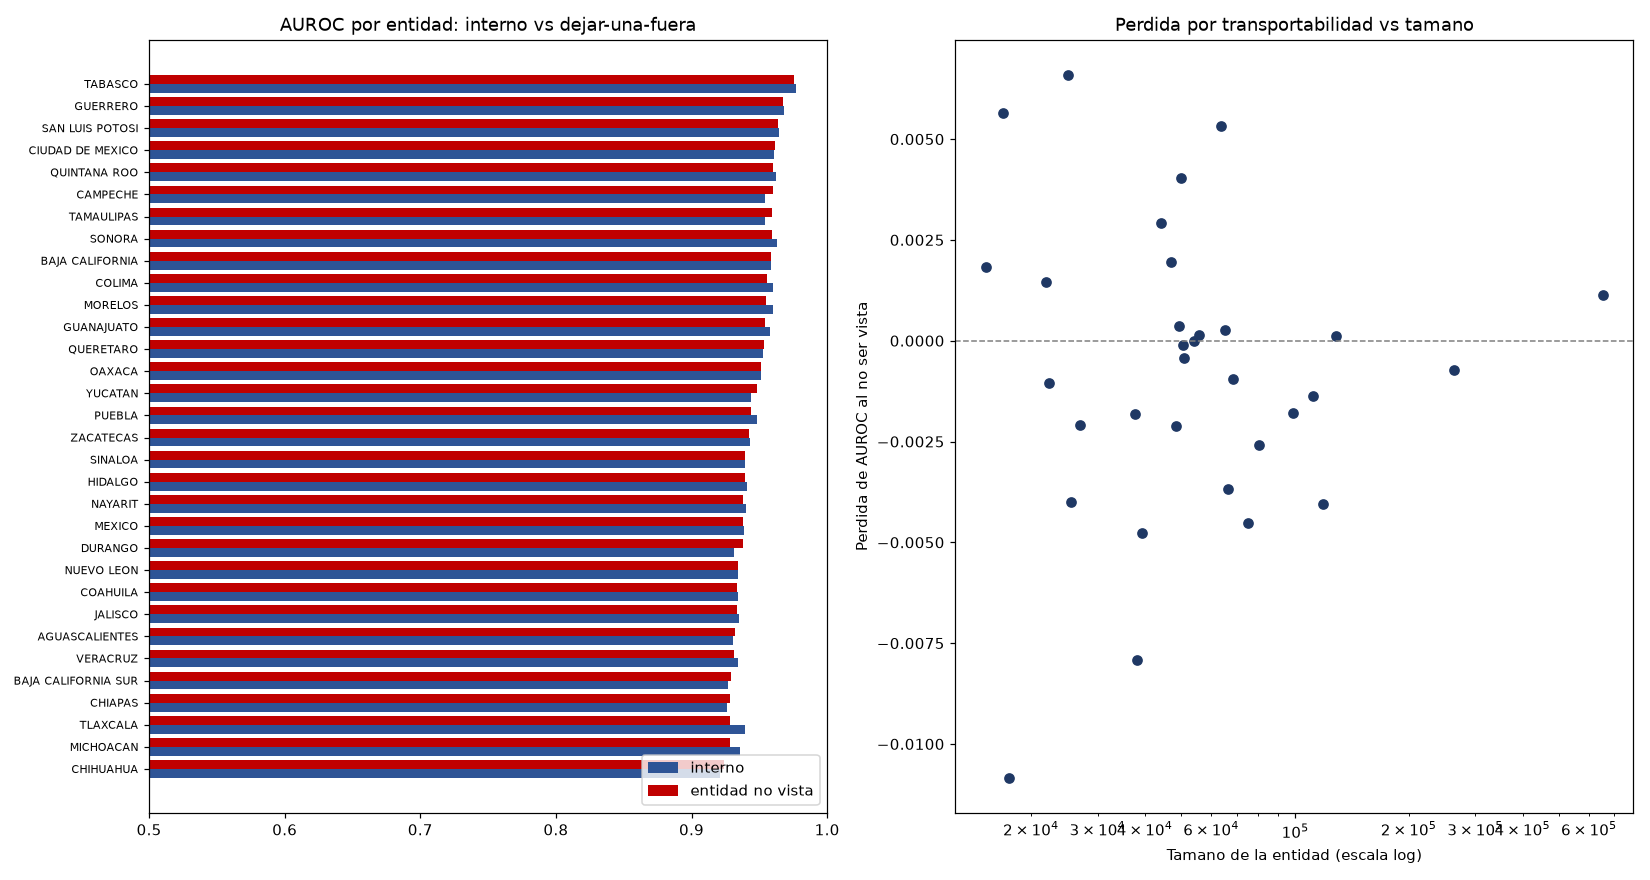
\includegraphics[width=\linewidth]{transportabilidad_loeo.png}
\caption{Transportabilidad geográfica interna. Izquierda: AUROC por entidad
habiendo participado en el entrenamiento frente a haber sido excluida.
Derecha: pérdida frente al tamaño de la entidad.}
\label{fig:loeo}
\end{figure}

\textbf{El desempeño se transfiere casi intacto.} La pérdida mediana de AUROC al
no haber visto la entidad es \loeoMediana, con un rango de $[\loeoMin,
\loeoMax]$: la entidad más afectada, \loeoPeor, pierde \loeoPeorDelta. De las
\loeoNent{} entidades, \loeoEmpeoran{} empeoran y el resto mejora; solo
\loeoMayoresUnPct{} supera una diferencia absoluta de 0.01.

\textbf{Las disparidades tampoco se acentúan.} La brecha de AUROC entre entidades
pasa de \loeoGapAurocInterno{} a \loeoGapAurocFuera{} y la de sensibilidad de
\loeoGapTprInterno{} a \loeoGapTprFuera: ambas se mantienen o se reducen
ligeramente.

El resultado tiene una lectura sustantiva que refuerza el argumento central. La
pérdida por transportabilidad no guarda relación con el tamaño de la entidad
($r=\loeoCorrTamr$, $p=\loeoCorrTamp$), de modo que el modelo no depende de haber
visto un estado concreto para funcionar en él. Combinado con el fracaso de la
reponderación (sección~\ref{sec:mitigacion_res}), esto cierra la explicación por
representación: la inequidad geográfica no proviene de que el modelo haya visto
pocos datos de ciertos estados --se comporta igual sin haber visto ninguno-- sino
de aplicar una regla de decisión común a poblaciones con distribuciones de riesgo
distintas.

La única asociación detectable es con la mortalidad de la entidad
($r=\loeoCorrTasar$, $p=\loeoCorrTasap$): los estados con más defunciones pierden
algo más al no haber sido vistos. Es la misma dirección que la correlación entre
AUROC y mortalidad de la sección~\ref{sec:correlatos}, y apunta al mismo
mecanismo pendiente de identificar.

\nota{Este diseño no sustituye a la validación externa. Que un modelo generalice
a un estado no visto \emph{de la misma fuente, el mismo año y el mismo proceso de
captura} dice poco sobre si generalizaría a otro sistema de registro. La
hipótesis~\ref{h4} sigue sin poner a prueba.}

\section{Mitigación de sesgo}
\label{sec:mitigacion_res}

La tabla~\ref{tab:mitigacion} compara las tres familias de intervención sobre el
mismo conjunto de prueba y el mismo punto de operación.

% Generado por generar_tablas.py -- NO editar a mano.

\begin{table}[htbp]
\centering
\caption{Comparación de las tres familias de mitigación sobre el conjunto de
prueba. Menor $\Delta$TPR indica mayor equidad entre entidades.}
\label{tab:mitigacion}
\small\setlength{\tabcolsep}{5pt}
\begin{tabular}{l r r r r}
\toprule
Intervención & $\Delta$TPR & $\Delta$FPR & Selec. & Exact.\ bal. \\
\midrule
Línea de base (umbral global) & 0.294 & 0.087 & 0.100 & 0.868 \\
Pre: reponderación por entidad & 0.290 & 0.082 & 0.099 & 0.865 \\
In: \emph{equalized odds} (Fairlearn)\textsuperscript{a} & 0.445 & -- & -- & -- \\
Post: umbral por entidad\textsuperscript{b} & 0.140 & 0.101 & 0.102 & 0.871 \\
Post: umbral por entidad (en muestra)\textsuperscript{c} & 0.022 & 0.107 & 0.101 & 0.869 \\
\bottomrule
\end{tabular}

\vspace{0.4em}
\begin{minipage}{0.95\linewidth}\footnotesize
\textsuperscript{a} Evaluado en una submuestra del bloque de entrenamiento
($n=\numprint{120000}$) y con un clasificador lineal; no es comparable uno a uno
con las demás filas. La reducción devuelve una distribución sobre clasificadores:
sobre 20 realizaciones del mismo modelo
ajustado, la brecha tiene mediana 0.397 y rango
[0.245, 0.628], intervalo
que contiene a la línea de base.\\
\textsuperscript{b} Umbrales estimados en el bloque de calibración y evaluados
en el de prueba: es la cifra desplegable.\\
\textsuperscript{c} Umbrales estimados sobre el propio conjunto de prueba:
cota optimista, reportada solo para dimensionar el sesgo de ajuste en muestra.
\end{minipage}
\end{table}


\subsection{Pre-procesamiento}

La reponderación inversa al tamaño de la entidad deja la brecha de sensibilidad
prácticamente intacta: \gapPre{} frente a \gapBase{} de la línea de base, con una
ligera pérdida de exactitud balanceada. El resultado es informativo: el problema
no es que el modelo haya visto pocos datos de las entidades pequeñas, sino que la
regla de decisión --un corte único-- interactúa mal con distribuciones de riesgo
heterogéneas. Reponderar la representación no puede corregir eso.

\subsection{In-procesamiento}

La reducción con restricción de \emph{equalized odds} arroja una brecha de
\gapIn, es decir, \emph{superior} a la de la línea de base. Pero el número
puntual no es lo relevante, y reportarlo solo sería engañoso.

La reducción por gradiente exponenciado no devuelve un clasificador, sino una
\emph{distribución} sobre clasificadores, de la que la predicción muestrea. Sobre
el mismo modelo ya ajustado y el mismo conjunto de evaluación,
\inRealizaciones{} realizaciones producen brechas con mediana \inMediana{} y
rango $[\inMin, \inMax]$. Ese intervalo contiene a la línea de base
(\gapBase) y es más ancho que cualquier efecto que pudiera atribuirse a la
restricción de equidad: la brecha depende más de qué realización toque que de la
intervención.

La interpretación correcta no es que el método sea inadecuado en general, sino
que resulta inestable en este régimen: con 32 grupos, algunos con pocos casos
positivos, el juego minimax que resuelve el algoritmo persigue la brecha máxima,
que en grupos pequeños está dominada por varianza de muestreo. A ello se suman las
limitaciones del montaje --submuestra y aprendiz lineal-- que impiden una
comparación uno a uno, como se advierte en la propia tabla.

\nota{Esta dispersión es también una advertencia de reproducibilidad. Si no se
fija la semilla en el momento de predecir --y no basta con fijarla al ajustar--,
el resultado del método cambia entre ejecuciones sin que nada lo señale. Un
trabajo que reportase una sola realización podría concluir tanto que la
intervención reduce la brecha como que la duplica.}

\subsection{Post-procesamiento}

El ajuste de umbrales por entidad es la única intervención efectiva. Con umbrales
estimados en el bloque de calibración y evaluados en el de prueba, la brecha de
sensibilidad cae de \gapBase{} a \gapPost, una reducción de \reduccionPost\,\%,
mientras la exactitud balanceada \emph{mejora} ligeramente, de \accBase{} a
\accPost, y la tasa de selección global se mantiene en torno a \selGlobal. Es decir: en
este problema la equidad geográfica se puede mejorar sustancialmente sin costo de
desempeño agregado.

\nota{La misma intervención, con umbrales estimados sobre el propio conjunto de
prueba, produce una brecha de \gapPostOpt. Esa cifra es una cota optimista y no
una política desplegable: mide qué tan bien se puede ajustar en retrospectiva, no
qué tan bien generalizaría. La diferencia entre \gapPostOpt{} y \gapPost{} --un
factor de \factorOptimismo-- dimensiona el sesgo que introduce estimar umbrales en
muestra, y es la razón por la que este trabajo reporta la segunda cifra como
resultado.}

\subsection{Frontera de Pareto}

La tabla~\ref{tab:pareto} y la figura~\ref{fig:pareto} presentan la frontera
obtenida interpolando entre el umbral global y los umbrales por entidad.

% Generado por generar_tablas.py -- NO editar a mano.

\begin{table}[htbp]
\centering
\caption{Frontera de Pareto equidad--desempeño. El parámetro $\alpha$ interpola
entre el umbral global ($\alpha=0$) y el umbral por entidad estimado fuera de
muestra ($\alpha=1$). Cada fila es una política de despliegue posible.}
\label{tab:pareto}
\begin{tabular}{r r r r}
\toprule
$\alpha$ & $\Delta$TPR & Exactitud balanceada & Selección \\
\midrule
0.0 & 0.2935 & 0.8680 & 0.1005 \\
0.1 & 0.2813 & 0.8672 & 0.0987 \\
0.2 & 0.2746 & 0.8664 & 0.0977 \\
0.3 & 0.2491 & 0.8667 & 0.0978 \\
0.4 & 0.2341 & 0.8693 & 0.0993 \\
0.5 & 0.2207 & 0.8713 & 0.1004 \\
0.6 & 0.2207 & 0.8706 & 0.0996 \\
0.7 & 0.2180 & 0.8700 & 0.0992 \\
0.8 & 0.2180 & 0.8703 & 0.0998 \\
0.9 & 0.1840 & 0.8695 & 0.0999 \\
1.0 & 0.1402 & 0.8711 & 0.1024 \\
\bottomrule
\end{tabular}
\end{table}


\begin{figure}[htbp]
\centering
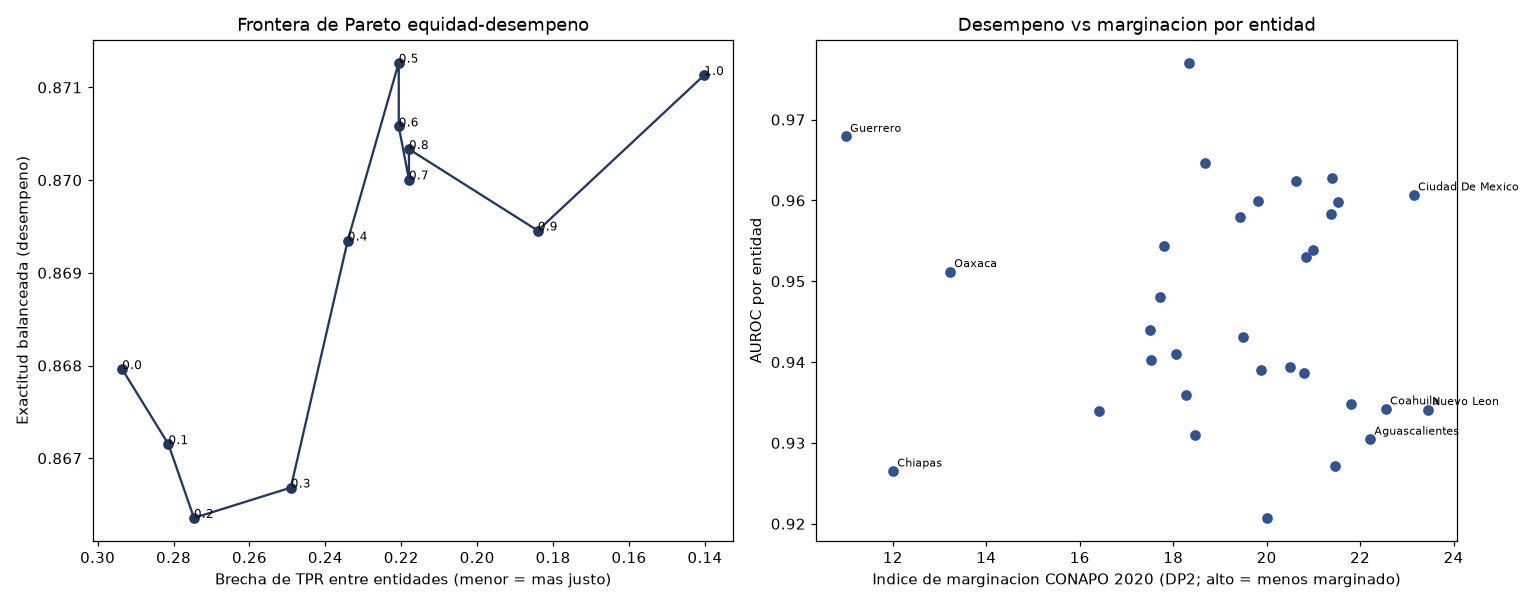
\includegraphics[width=\linewidth]{pareto_mitigacion.png}
\caption{Frontera de Pareto equidad--desempeño (izquierda) y desempeño por entidad
frente al índice de marginación de CONAPO 2020 (derecha; un valor más alto indica
menor marginación).}
\label{fig:pareto}
\end{figure}

La forma de la frontera es el resultado con mayor valor práctico: la exactitud
balanceada permanece en la banda \paretoAccMin--\paretoAccMax{} a lo largo de todo
el recorrido, mientras la brecha de sensibilidad desciende de \paretoGapMax{} a
\paretoGapMin. No hay, en este
problema, un intercambio material entre equidad y desempeño agregado; la
resistencia a corregir la disparidad no puede justificarse invocando pérdida de
utilidad clínica global.

Conviene señalar que el descenso no es monótono ni suave: entre $\alpha=0.5$ y
$\alpha=0.8$ la brecha se estanca en torno a
\paretoMesetaMin--\paretoMesetaMax. Ese estancamiento
refleja que la brecha máxima está determinada por unas pocas entidades extremas, y
que la interpolación lineal solo las alcanza cuando $\alpha$ se aproxima a 1.
Para el despliegue, la lectura es que las políticas intermedias rinden menos de lo
que sugeriría una interpolación proporcional.
